\documentclass{standalone}
\usepackage{tikz}
\usetikzlibrary{patterns, positioning}

\begin{document}
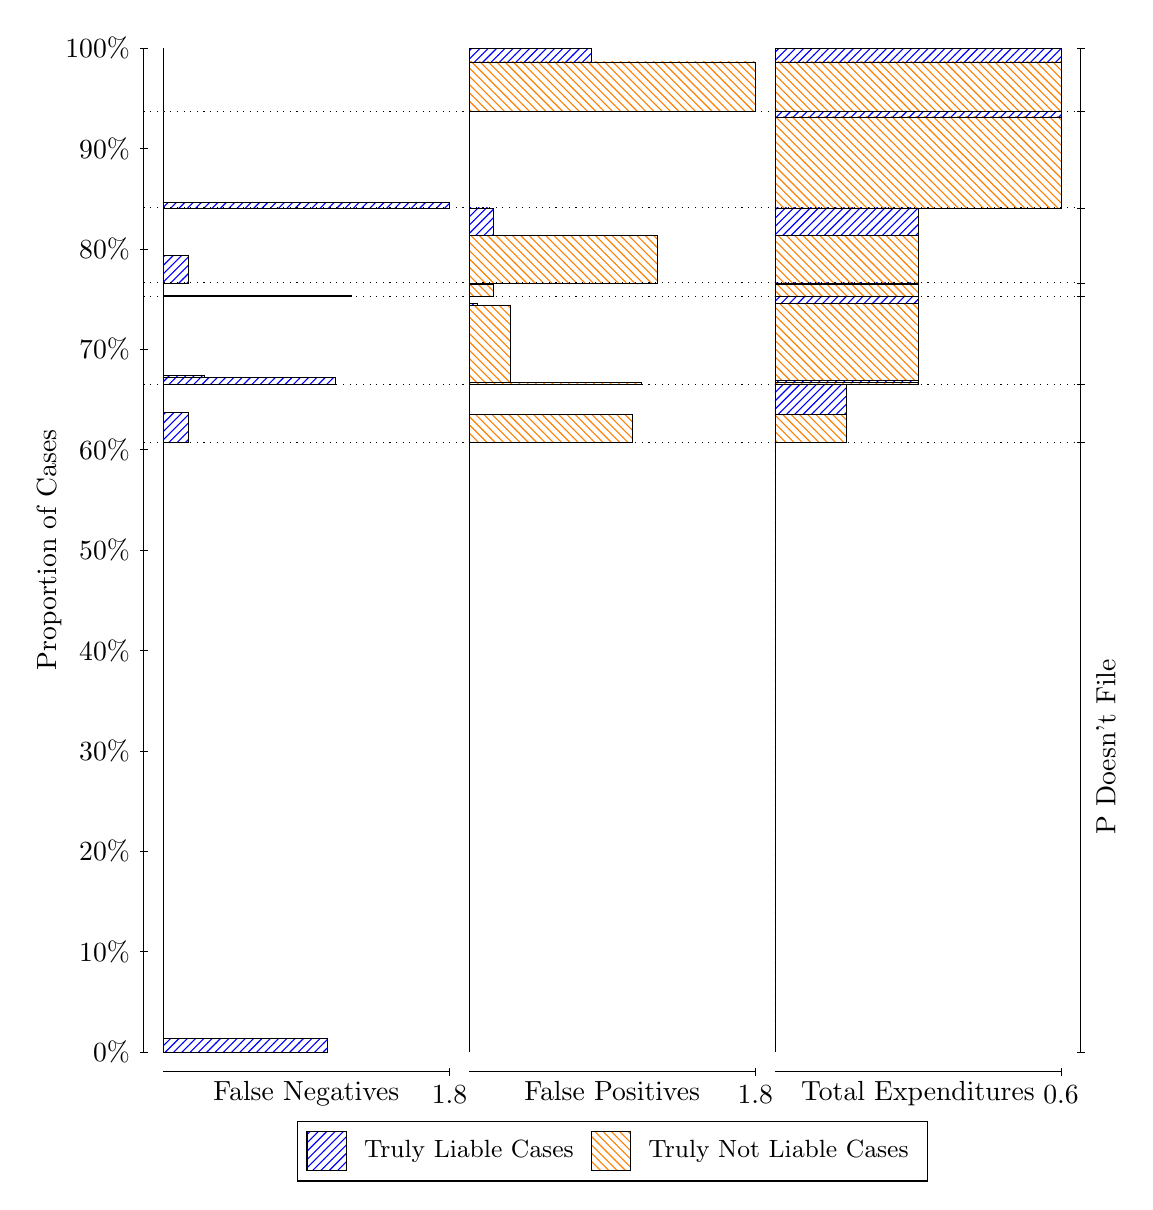
\begin{tikzpicture}
\draw[black, very thin] (1.5,1.75) -- (1.5,14.5);
\node[rotate=90, anchor=center] at (0.3, 8.125) {Proportion of Cases};
\draw[black, very thin] (1.45,1.75) -- (1.55,1.75);
\node[anchor=east] at (1.45, 1.75) {0\%};
\draw[black, very thin] (1.45,3.025) -- (1.55,3.025);
\node[anchor=east] at (1.45, 3.025) {10\%};
\draw[black, very thin] (1.45,4.3) -- (1.55,4.3);
\node[anchor=east] at (1.45, 4.3) {20\%};
\draw[black, very thin] (1.45,5.575) -- (1.55,5.575);
\node[anchor=east] at (1.45, 5.575) {30\%};
\draw[black, very thin] (1.45,6.85) -- (1.55,6.85);
\node[anchor=east] at (1.45, 6.85) {40\%};
\draw[black, very thin] (1.45,8.125) -- (1.55,8.125);
\node[anchor=east] at (1.45, 8.125) {50\%};
\draw[black, very thin] (1.45,9.4) -- (1.55,9.4);
\node[anchor=east] at (1.45, 9.4) {60\%};
\draw[black, very thin] (1.45,10.675) -- (1.55,10.675);
\node[anchor=east] at (1.45, 10.675) {70\%};
\draw[black, very thin] (1.45,11.95) -- (1.55,11.95);
\node[anchor=east] at (1.45, 11.95) {80\%};
\draw[black, very thin] (1.45,13.225) -- (1.55,13.225);
\node[anchor=east] at (1.45, 13.225) {90\%};
\draw[black, very thin] (1.45,14.5) -- (1.55,14.5);
\node[anchor=east] at (1.45, 14.5) {100\%};

\draw[black, very thin] (13.4,1.75) -- (13.4,14.5);
\draw[black, very thin] (13.35,1.75) -- (13.45,1.75);
\node[anchor=west] at (13.35, 1.75) {};
\draw[black, very thin] (13.35,9.4955) -- (13.45,9.4955);
\node[anchor=west] at (13.35, 9.4955) {};
\draw[black, very thin] (13.35,10.23) -- (13.45,10.23);
\node[anchor=west] at (13.35, 10.23) {};
\draw[black, very thin] (13.35,11.344) -- (13.45,11.344);
\node[anchor=west] at (13.35, 11.344) {};
\draw[black, very thin] (13.35,11.518) -- (13.45,11.518);
\node[anchor=west] at (13.35, 11.518) {};
\draw[black, very thin] (13.35,12.471) -- (13.45,12.471);
\node[anchor=west] at (13.35, 12.471) {};
\draw[black, very thin] (13.35,13.696) -- (13.45,13.696);
\node[anchor=west] at (13.35, 13.696) {};
\draw[black, very thin] (13.35,14.5) -- (13.45,14.5);
\node[anchor=west] at (13.35, 14.5) {};

\draw[black, very thin, pattern color=blue, pattern=north east lines] (1.75,1.75) rectangle (3.8262,1.9249);
\draw[black, very thin, pattern color=orange, pattern=north west lines] (1.75,1.9249) rectangle (1.75,9.4955);
\draw[black, very thin, pattern color=blue, pattern=north east lines] (1.75,9.4955) rectangle (2.0614,9.876);
\draw[black, very thin, pattern color=orange, pattern=north west lines] (1.75,9.876) rectangle (1.75,10.23);
\draw[black, very thin, pattern color=blue, pattern=north east lines] (1.75,10.23) rectangle (3.93,10.318);
\draw[black, very thin, pattern color=blue, pattern=north east lines] (1.75,10.318) rectangle (3.7224,10.318);
\draw[black, very thin, pattern color=blue, pattern=north east lines] (1.75,10.318) rectangle (3.5148,10.318);
\draw[black, very thin, pattern color=blue, pattern=north east lines] (1.75,10.318) rectangle (3.3071,10.318);
\draw[black, very thin, pattern color=blue, pattern=north east lines] (1.75,10.318) rectangle (3.0995,10.32);
\draw[black, very thin, pattern color=blue, pattern=north east lines] (1.75,10.32) rectangle (2.8919,10.32);
\draw[black, very thin, pattern color=blue, pattern=north east lines] (1.75,10.32) rectangle (2.6843,10.32);
\draw[black, very thin, pattern color=blue, pattern=north east lines] (1.75,10.32) rectangle (2.4767,10.32);
\draw[black, very thin, pattern color=blue, pattern=north east lines] (1.75,10.32) rectangle (2.269,10.344);
\draw[black, very thin, pattern color=orange, pattern=north west lines] (1.75,10.344) rectangle (1.75,11.344);
\draw[black, very thin, pattern color=blue, pattern=north east lines] (1.75,11.344) rectangle (4.1376,11.357);
\draw[black, very thin, pattern color=orange, pattern=north west lines] (1.75,11.357) rectangle (1.75,11.518);
\draw[black, very thin, pattern color=blue, pattern=north east lines] (1.75,11.518) rectangle (2.0614,11.866);
\draw[black, very thin, pattern color=orange, pattern=north west lines] (1.75,11.866) rectangle (1.75,12.471);
\draw[black, very thin, pattern color=blue, pattern=north east lines] (1.75,12.471) rectangle (5.3833,12.541);
\draw[black, very thin, pattern color=orange, pattern=north west lines] (1.75,12.541) rectangle (1.75,13.696);
\draw[black, very thin, pattern color=orange, pattern=north west lines] (1.75,13.696) rectangle (1.75,14.324);
\draw[black, very thin, pattern color=blue, pattern=north east lines] (1.75,14.324) rectangle (1.75,14.5);
\draw[black, very thin, pattern color=orange, pattern=north west lines] (5.6333,1.75) rectangle (5.6333,9.3206);
\draw[black, very thin, pattern color=blue, pattern=north east lines] (5.6333,9.3206) rectangle (5.6333,9.4955);
\draw[black, very thin, pattern color=orange, pattern=north west lines] (5.6333,9.4955) rectangle (7.7095,9.8495);
\draw[black, very thin, pattern color=blue, pattern=north east lines] (5.6333,9.8495) rectangle (5.6333,10.23);
\draw[black, very thin, pattern color=orange, pattern=north west lines] (5.6333,10.23) rectangle (7.8133,10.251);
\draw[black, very thin, pattern color=orange, pattern=north west lines] (5.6333,10.251) rectangle (7.6057,10.251);
\draw[black, very thin, pattern color=orange, pattern=north west lines] (5.6333,10.251) rectangle (7.3981,10.251);
\draw[black, very thin, pattern color=orange, pattern=north west lines] (5.6333,10.251) rectangle (7.1905,10.251);
\draw[black, very thin, pattern color=orange, pattern=north west lines] (5.6333,10.251) rectangle (6.9829,10.255);
\draw[black, very thin, pattern color=orange, pattern=north west lines] (5.6333,10.255) rectangle (6.7752,10.255);
\draw[black, very thin, pattern color=orange, pattern=north west lines] (5.6333,10.255) rectangle (6.7752,10.255);
\draw[black, very thin, pattern color=orange, pattern=north west lines] (5.6333,10.255) rectangle (6.5676,10.255);
\draw[black, very thin, pattern color=orange, pattern=north west lines] (5.6333,10.255) rectangle (6.36,10.255);
\draw[black, very thin, pattern color=orange, pattern=north west lines] (5.6333,10.255) rectangle (6.1524,11.23);
\draw[black, very thin, pattern color=blue, pattern=north east lines] (5.6333,11.23) rectangle (5.7371,11.255);
\draw[black, very thin, pattern color=blue, pattern=north east lines] (5.6333,11.255) rectangle (5.6333,11.344);
\draw[black, very thin, pattern color=orange, pattern=north west lines] (5.6333,11.344) rectangle (5.9448,11.506);
\draw[black, very thin, pattern color=blue, pattern=north east lines] (5.6333,11.506) rectangle (5.6333,11.518);
\draw[black, very thin, pattern color=orange, pattern=north west lines] (5.6333,11.518) rectangle (8.021,12.124);
\draw[black, very thin, pattern color=blue, pattern=north east lines] (5.6333,12.124) rectangle (5.9448,12.471);
\draw[black, very thin, pattern color=orange, pattern=north west lines] (5.6333,12.471) rectangle (5.6333,13.626);
\draw[black, very thin, pattern color=blue, pattern=north east lines] (5.6333,13.626) rectangle (5.6333,13.696);
\draw[black, very thin, pattern color=orange, pattern=north west lines] (5.6333,13.696) rectangle (9.2667,14.324);
\draw[black, very thin, pattern color=blue, pattern=north east lines] (5.6333,14.324) rectangle (7.1905,14.5);
\draw[black, very thin, pattern color=orange, pattern=north west lines] (9.5167,1.75) rectangle (9.5167,9.3206);
\draw[black, very thin, pattern color=blue, pattern=north east lines] (9.5167,9.3206) rectangle (9.5167,9.4955);
\draw[black, very thin, pattern color=orange, pattern=north west lines] (9.5167,9.4955) rectangle (10.425,9.8495);
\draw[black, very thin, pattern color=blue, pattern=north east lines] (9.5167,9.8495) rectangle (10.425,10.23);
\draw[black, very thin, pattern color=orange, pattern=north west lines] (9.5167,10.23) rectangle (11.333,10.255);
\draw[black, very thin, pattern color=blue, pattern=north east lines] (9.5167,10.255) rectangle (11.333,10.281);
\draw[black, very thin, pattern color=orange, pattern=north west lines] (9.5167,10.281) rectangle (11.333,11.256);
\draw[black, very thin, pattern color=blue, pattern=north east lines] (9.5167,11.256) rectangle (11.333,11.344);
\draw[black, very thin, pattern color=orange, pattern=north west lines] (9.5167,11.344) rectangle (11.333,11.344);
\draw[black, very thin, pattern color=blue, pattern=north east lines] (9.5167,11.344) rectangle (11.333,11.344);
\draw[black, very thin, pattern color=orange, pattern=north west lines] (9.5167,11.344) rectangle (11.333,11.506);
\draw[black, very thin, pattern color=blue, pattern=north east lines] (9.5167,11.506) rectangle (11.333,11.518);
\draw[black, very thin, pattern color=orange, pattern=north west lines] (9.5167,11.518) rectangle (11.333,12.124);
\draw[black, very thin, pattern color=blue, pattern=north east lines] (9.5167,12.124) rectangle (11.333,12.471);
\draw[black, very thin, pattern color=orange, pattern=north west lines] (9.5167,12.471) rectangle (13.15,13.626);
\draw[black, very thin, pattern color=blue, pattern=north east lines] (9.5167,13.626) rectangle (13.15,13.696);
\draw[black, very thin, pattern color=orange, pattern=north west lines] (9.5167,13.696) rectangle (13.15,14.324);
\draw[black, very thin, pattern color=blue, pattern=north east lines] (9.5167,14.324) rectangle (13.15,14.5);
\draw[black, dotted] (1.5,9.4955) -- (13.4,9.4955);
\draw[black, dotted] (1.5,10.23) -- (13.4,10.23);
\draw[black, dotted] (1.5,11.344) -- (13.4,11.344);
\draw[black, dotted] (1.5,11.518) -- (13.4,11.518);
\draw[black, dotted] (1.5,12.471) -- (13.4,12.471);
\draw[black, dotted] (1.5,13.696) -- (13.4,13.696);
\draw[black, very thin] (1.75,1.5) -- (5.3833,1.5);
\node[anchor=north] at (3.5667, 1.5) {False Negatives};
\draw[black, very thin] (5.3833,1.45) -- (5.3833,1.55);
\node[anchor=north] at (5.3833, 1.45) {1.8};

\draw[black, very thin] (5.6333,1.5) -- (9.2667,1.5);
\node[anchor=north] at (7.45, 1.5) {False Positives};
\draw[black, very thin] (9.2667,1.45) -- (9.2667,1.55);
\node[anchor=north] at (9.2667, 1.45) {1.8};

\draw[black, very thin] (9.5167,1.5) -- (13.15,1.5);
\node[anchor=north] at (11.333, 1.5) {Total Expenditures};
\draw[black, very thin] (13.15,1.45) -- (13.15,1.55);
\node[anchor=north] at (13.15, 1.45) {0.6};

\node[black, centered, rotate=90] at (13.72, 5.6227) {P Doesn't File};







\draw (7.449999999999999,1.5) node[draw=none] (baseCoordinate) {};
\begin{scope}[align=center]
        \matrix[scale=0.5, draw=black, below=0.5cm of baseCoordinate, nodes={draw}, column sep=0.1cm]{
            \node[rectangle, draw, minimum width=0.5cm, minimum height=0.5cm, pattern=north east lines, pattern color=blue] {}; &
            \node[draw=none, font=\small] (B) {Truly Liable Cases}; &
            \node[rectangle, draw, minimum width=0.5cm, minimum height=0.5cm, pattern=north west lines, pattern color=orange] {}; &
            \node[draw=none, font=\small] (B) {Truly Not Liable Cases}; \\
            };
\end{scope}

\end{tikzpicture}
\end{document}